\chapter{Subject of the thesis}
\label{chapter:3_subject}

\section{Test application}
\label{chapter:3_test_app}
For the purpose of getting familiar with the techniques and testing them, a test application was created. It allows a user to switch between implemented rendering techniques and observe their effects in an interactive first-person scene.

The application was written in the C++ programming language. It uses the Win32 platform to create windows in a Windows operating system. It uses DirectX 12 to utilize the GPU for rendering graphics. DirectX 12 was chosen because it is the newest of DirectX versions, allowing for granular control over the rendering process and boasting advanced features. It is also very widely adopted for all sorts of computer graphics tasks, making it worth specializing in. Additionally, the DirectX 12 API is much more verbose and involved as compared to, for example, OpenGL, which forces the programmer to gain more in-depth knowledge about graphics programming and all the processes involved.

Two notable open-source libraries were utilized in the project. Dear ImGui is a library simplifying the creation of graphical user interfaces. It is compatible with all the major graphics programming APIs, including DX12, making it fast and easy to integrate into a project, providing am intuitive and smooth user experience at the same time. The other library is the Tracy Profiler. The instrumentation library is just a part of the Tracy ecosystem, with separate applications like the profiler to gather and analyze performance data. It is simple to incorporate into an existing project and very performant, adding almost no overhead. Code zones and frames that will be captured when profiling are marked manually by the programmer, giving them full control over what data is captured. This also improves the readability of the outputs, which stands in contrast with other profilers that automatically gather data and can easily overwhelm the user and clutter the presentation with the amount of information provided.

The project uses CMake to fetch all the project dependencies and create a buildable MSVC project.

\section{Implemented shadow rendering techniques}
In the following sections, all the shadow rendering techniques that have been implemented during work on this thesis are described, along with explanations of their algorithms.

\subsection{Planar shadows implementation}
\label{section:planar_shadows_impl}

Planar shadows, as described in section \ref{section:planar_shadows}, are a very simple technique to achieve hard shadows, introduced by Blinn \cite{bib:article:blinn_shadows}. The idea for the algorithm stems from the geometric understanding of how a shadow is formed. The shape of a shadow is basically the shadow caster projected onto the surface of a shadow receiver along rays from a light source, as shown in Fig. \ref{fig:projection_shadow}. 

\begin{figure}[h]
	\centering
	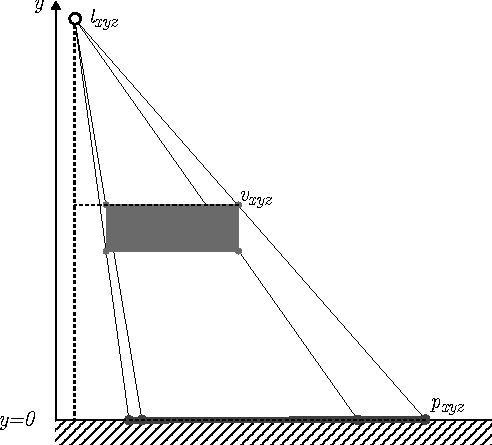
\includegraphics[width=0.5\textwidth]{./graf/projection_shadow.pdf}
	\caption{Vertices of a shadow caster projected onto \(y=0\) plane create a planar shadow. Dashed lines visualize the similar triangles.}
	\label{fig:projection_shadow}
\end{figure}

Using this geometric understanding and similar triangles, marked in Fig. \ref{fig:projection_shadow} in dashed lines, the following equations and a projection matrix can be derived. Assuming \(l\) to be the position of a light source, \(v\) to be the position of a vertex of the shadow caster and \(p\) the position of the projected shadow vertex, a projection onto the \(y=0\) plane is described by:
\begin{align}
	\frac{p_x - l_x}{v_x - l_x} = \frac{l_y}{l_y - v_y} \Longleftrightarrow p_x = \frac{l_yv_x - l_xv_y}{l_y - v_y}
\end{align}
The \(z\) component is derived in analogous way:
\begin{align}
	\frac{p_z - l_z}{v_z - l_z} = \frac{l_y}{l_y - v_y} \Longleftrightarrow p_z = \frac{l_yv_z - l_zv_y}{l_y - v_y}
\end{align}
The \(y\) component will be \(y=0\) since the projection happens onto the \(xz\) plane. From that the projection matrix can be constructed:
\begin{align}
	\mathbf{M} = 
	\begin{pmatrix}
		l_y & -l_x & 0 & 0\\
		0 & 0 & 0 & 0\\
		0 & -l_z & l_y & 0\\
		0 & -1 & 0 & l_y
	\end{pmatrix}
\end{align}
The \(l_y - v_y\) factor in the denominator is obtained by utilizing the property of homogenous coordinates, where all components of a vector \(\mathbf{v} = \begin{bmatrix}x & y & z & w\end{bmatrix}^T\) get divided by the \(w\) component, which gives \(\mathbf{v} = \begin{bmatrix}x/w & y/w & z/w & 1\end{bmatrix}^T\).

This matrix can be generalized to project points onto any plane, but this was not implemented.

In the implementation the matrix is created in the vertex shader based on the position of the light source. The vertices of the caster, after being transformed into world space, are multiplied by it, projecting them onto the \(y=0\) plane. Then they are transformed with the view and perspective projection matrices as usual. The resulting mesh is rendered in black, with a pixel shader that just returns the black color. Special care should be taken when rendering the shadow mesh, since it perfectly overlaps the ground plane at \(y=0\). To avoid z-fighting, which is shown in Fig \ref{fig:projection_shadow_beyond}, this mesh needs to be rendered after the receiver and before the caster, with z depth testing turned off in the rendering pipeline, or, as is the case in the implementation, a negative depth offset needs to be added to the mesh to bring it above the ground plane.

\begin{figure}[h]
    \centering
    \begin{subfigure}[t]{0.45\textwidth}
		\centering
        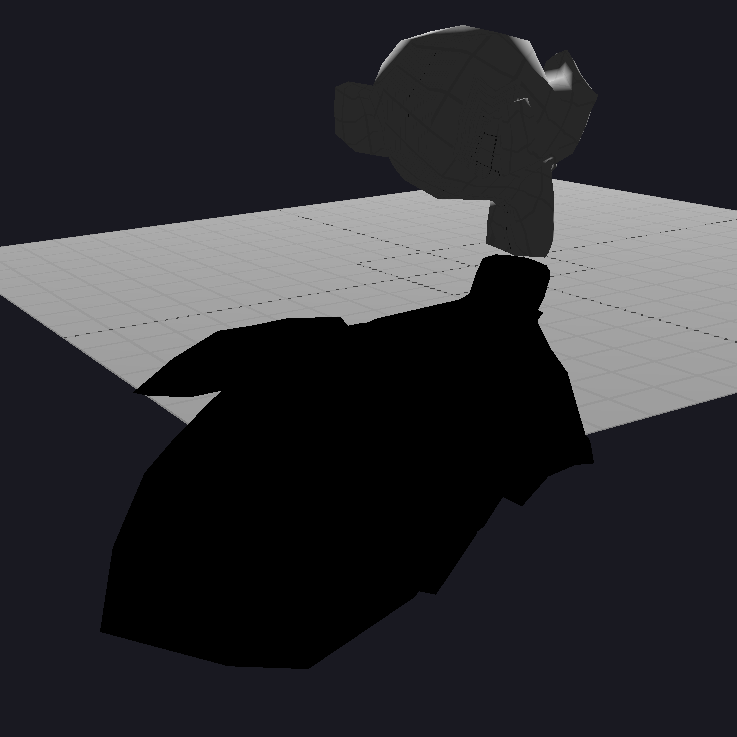
\includegraphics[width=\textwidth]{./graf/projection_shadow_beyond.png}
        \caption{The projected shadow mesh lies beyond the ground plane.}
        \label{fig:projection_shadow_beyond}
    \end{subfigure}
	\hfill
    \begin{subfigure}[t]{0.45\textwidth}
		\centering
        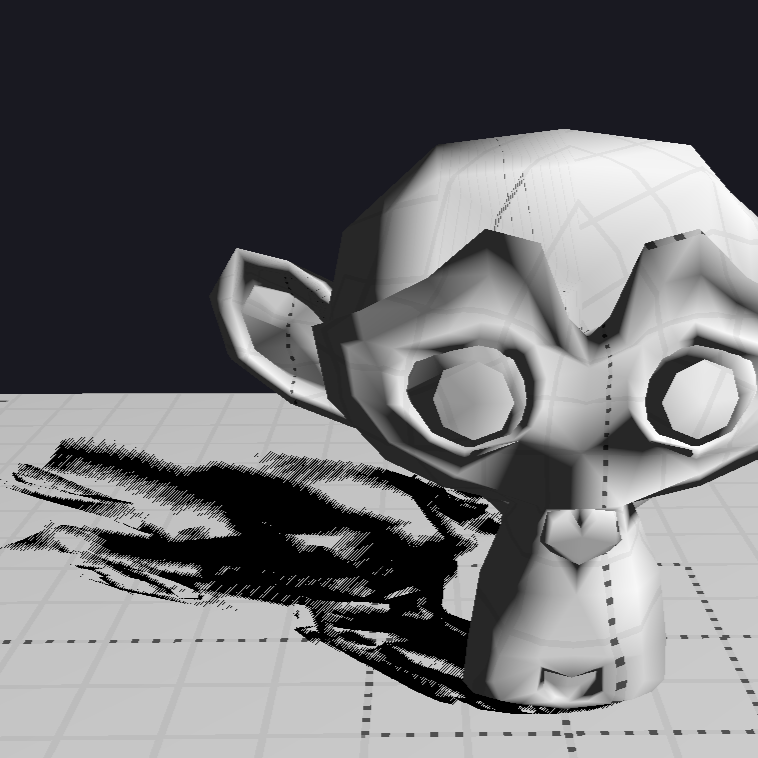
\includegraphics[width=\textwidth]{./graf/projection_shadow_fighting.png}
        \caption{Severe z-fighting caused by the fact that both the ground plane mesh and shadow mesh lie in the exact same plane.}
        \label{fig:projection_shadow_fighting}
    \end{subfigure}

    \caption{Some of the issues that can arise when using projection shadows.}
    \label{fig:projection_shadow_issues}
\end{figure}

Multiple issues arise with this technique. The receiver must be a flat plane, objects cannot shadow themselves, casters and receivers need separate treatment. Additionally, care needs to be taken to only render the shadow meshes on top of the geometry of a receiver. Since the shadow is a separate mesh, it could be cast beyond the actual surface of the receiver, creating an impossible shadow in the air. This is illustrated in Fig \ref{fig:projection_shadow_fighting} There is another possibility here for an impossible shadow. If the light source is between the caster and receiver, an anti-shadow will be cast as shown in Fig \ref{fig:projection_anti_shadow}. This creates another special case that needs to be checked for by the application. Soft shadows are also difficult and costly to achieve, created by projecting the caster geometry multiple times using different discrete locations sampled over the area of the light source. The shadow meshes can then be blended, producing a darker color where more shadows are present. This gives very accurate results with a high number of samples, but is not a viable option for real-time rendering. All these problems make this technique virtually unused in modern rendering engines.
\begin{figure}[hb]
	\centering
	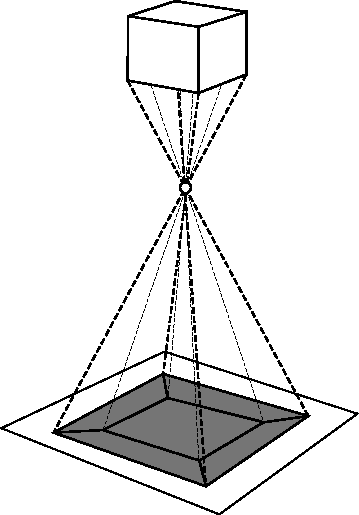
\includegraphics[width=0.35\textwidth]{./graf/projection_anti_shadow.pdf}
	\caption{The shadow caster projected through a light source, creating an anti-shadow.}
	\label{fig:projection_anti_shadow}
\end{figure}

% TODO: add some notes on performance.

\subsection{Implementation of basic shadow mapping}
\label{section:basic_mapping_impl}
As mentioned in chapter \ref{section:basic_mapping}, shadow mapping for a single light source is performed using two render passes. The first one generates the shadow map itself, the second and final pass renders the scene with shadows determined using the shadow map. The shadow map is a z-buffer, which means that, for each texel, it stores the values of the z coordinate of the scene surface point being rendered. These coordinates are stored after transforming the vertices of the scene into the NDC space, or normalized device coordinate space, of a given light source. This transformation is achieved in the vertex shader, by using the regular world, view, projection (WVP) transformation matrices, with the distinction that the view and projection matrices are not of the scene observer but of the light source. In truth, multiplying the vertex positions by the WVP matrix will result in clip space homogenous coordinates, which then will be transformed automatically by the pipeline into NDC during the perspective division, when the homogenous coordinates are divided by their \(w\) component. The stored depth values will then be in the \(0-1\) range, usually \(0\) being at the near clipping plane and \(1\) at the far clipping plane. This z-buffer can then be used as a texture shader resource in a pixel shader to render the final scene. To read the depth values from the shadow map, the NDC coordinates of each surface point need to be calculated again. The \(x\) any \(y\) components will then be used to access a texel in the shadow map, the \(z\) component will be compared with the contents of the shadow map. Do note that the actual Euclidean distance between the shaded point and the light source is not used, as these values would be in different coordinate spaces. When the shadow map value is accessed, it is compared with the \(z\) value of the point that is currently being shaded. If the shadow map value is greater, then the point being shaded is farther away from the light source than some other surface seen at this point from the point of view of the light. This means that it is not illuminated and is in shadow. Otherwise, the point is lit by the light source. The process is illustrated in Fig. \ref{fig:shadow_map_basic}. Fig. \ref{fig:shadow_map_screens} shows a rendered view of a scene with shadow mapping and the shadow map itself.
\begin{figure}[h]
	\centering
	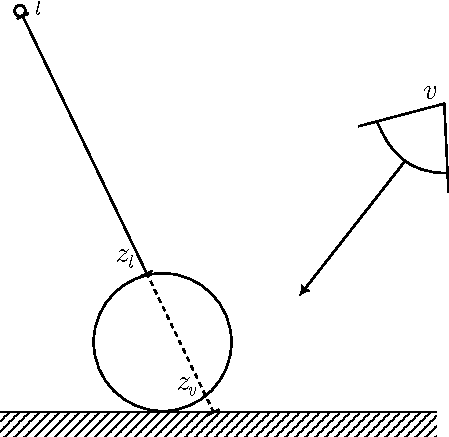
\includegraphics[width=0.6\textwidth]{./graf/shadow_mapping_basic.pdf}
	\caption{The light source \(l\) has stored the depth value \(z_l\) in its shadow map. When rendering the scene from the viewpoint of the observer \(v\), the stored depth is compared to the depth \(z_v\). This value will be larger than the one in the shadow map, so the point will be in shadow.}
	\label{fig:shadow_map_basic}
\end{figure}

\begin{figure}[ht]
    \centering
    \begin{subfigure}{0.45\textwidth}
		\centering
        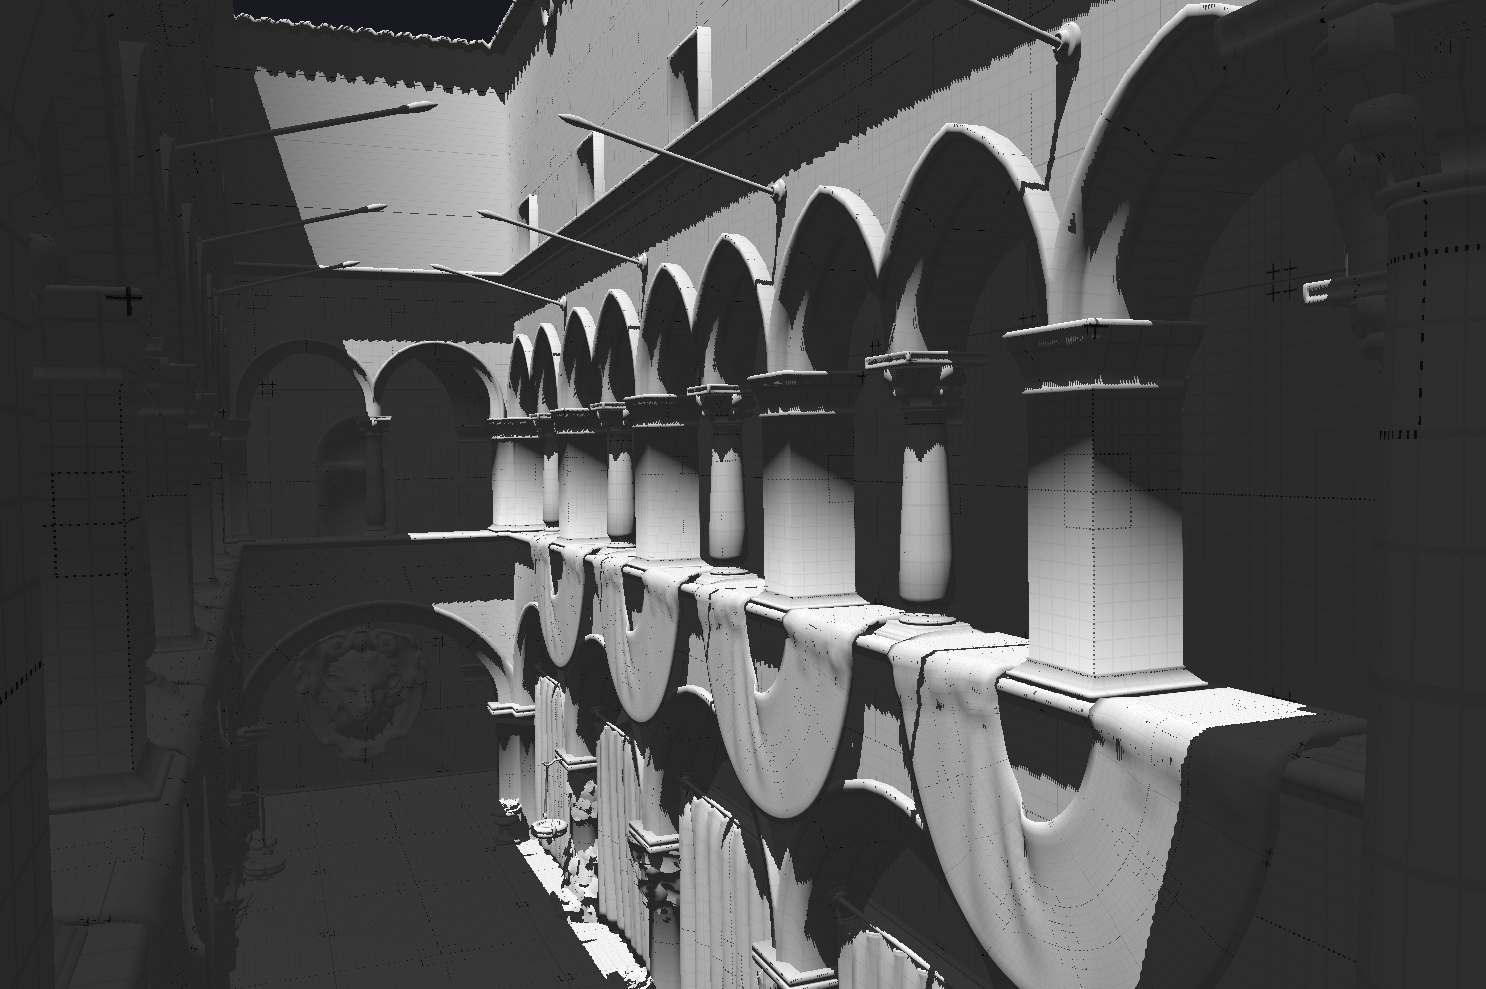
\includegraphics[width=\textwidth]{./graf/shadow_mapping_basic_sponza.png}
        \caption{A scene rendered with the use of shadow mapping.}
        \label{fig:shadow_map_screens_scene}
    \end{subfigure}
	\hfill
    \begin{subfigure}{0.45\textwidth}
		\centering
        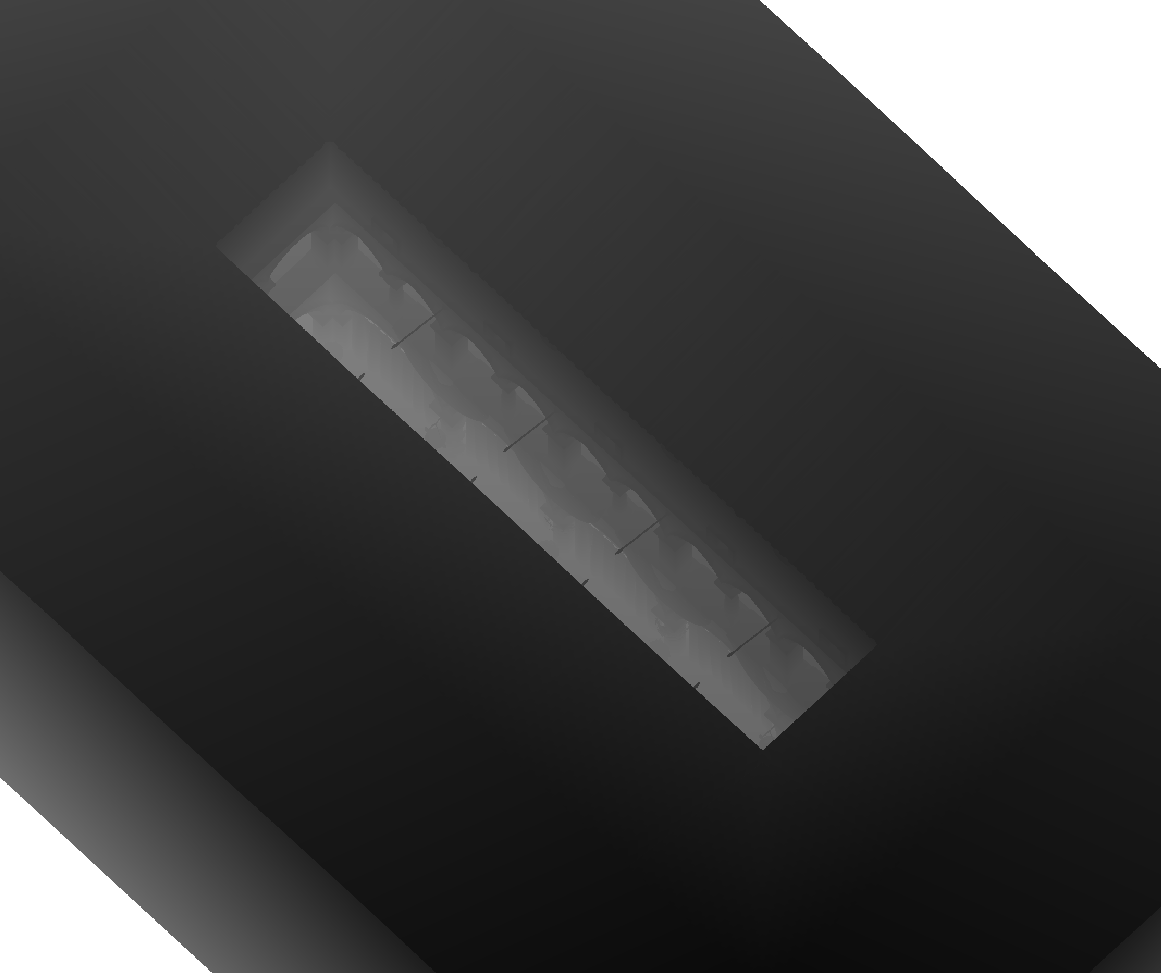
\includegraphics[width=\textwidth]{./graf/shadow_mapping_basic_depth_map.png}
        \caption{Section of the shadow map rendered for this scene.}
        \label{fig:shadow_map_screens_depth}
    \end{subfigure}

    \caption{An example scene rendered with a shadow map, which is shown in black and white.}
    \label{fig:shadow_map_screens}
\end{figure}

To implement this technique a resource is needed that will be used both as an additional depth buffer and a texture. This can be easily achieved in an application programming interface (API) like DirectX 12 by creating one resource and two resource views, one being a Depth Stencil View (DSV) and another a Shader resource view (SRV). Once the rendering of the shadow map is finished using the DSV, the resource can be transitioned in preparation to be used as an SRV during rendering the main view using a resource barrier. Caution needs to be taken to transition the resource back to a DSV-compatible state before rendering the shadow map of the next frame. In this case, a resource barrier will also ensure that all write operations have finished before continuing with rendering, meaning that the rendering of the shadow map will be complete before it is used in the final pass. The shaders responsible for rendering the main scene view will evidently need access to the texture resource containing the shadow map, but also it will need to access the view and projection matrices of the light view pass. This is to calculate the corresponding NDC coordinates of the point being shaded in the shadow map. It is optimal to calculate light clip space coordinates in the vertex shader and let the pipeline interpolate them across the triangle for each fragment. Since the perspective division will not happen automatically here, it is needed to divide the coordinates by the \(w\) component in the pixel shader to obtain correct NDC values. Since the shadow map is sampled as a texture, the \(xy\) coordinates with range \([-1:1]\) need to be converted into \(uv\) texture coordinates with range \([0:1]\). Additionally, the \(y\) component needs to be flipped to address the texture correctly. This can be performed as a simple transformation in the pixel shader as \(\begin{bmatrix}x & y\end{bmatrix}^T /  \begin{bmatrix}2 & -2\end{bmatrix}^T + \begin{bmatrix}0.5 & 0.5\end{bmatrix}^T\) or incorporated into the MVP matrix of the light view. This can be achieved by multiplying the MVP matrix for the light source by the offset matrix as shown in equation \ref{eq:offset_matrix_shadow_mapping}.

\begin{align}
	\label{eq:offset_matrix_shadow_mapping}
	\mathbf{L_{offset}} = 
	\begin{pmatrix}
		0.5 & 0 & 0 & 0.5\\
		0 & -0.5 & 0 & 0.5\\
		0 & 0 & 1 & 0\\
		0 & 0 & 0 & 1
	\end{pmatrix}
	\cdot \mathbf{MVP}
\end{align}

When sampling the shadow map as a texture, it is important to do so with a sampler that does not perform any filtering on the texture. Typically, texture filtering helps avoid different kinds of aliasing. Regular color textures however can be filtered and interpolated as they only store color data. The shadow map, which stores depth values, cannot be filtered in the same way as the produced values would be senseless in this process. They would create non-existing apparent surfaces especially noticeable between sharp depth changes, for example between a close object and the far clipping plane.

This observation brings forth one of the issues with shadow mapping: they cannot be filtered to avoid aliasing. One could also attempt to blur a shadow map to achieve soft shadows, but this is not a viable option for the same reason. Because of this basic shadow mapping can only be used to create hard shadows that suffer from aliasing issues, creating shadows that can appear blocky when up close, as in Fig. \ref{fig:shadow_mapping_blocky}. Aliasing can be mitigated by rendering the shadow map into a higher resolution target, but only to a degree. Special techniques allowing for smoothing and filtering shadows generated with shadow mapping will be presented in the following sections.
\begin{figure}[h]
    \centering
	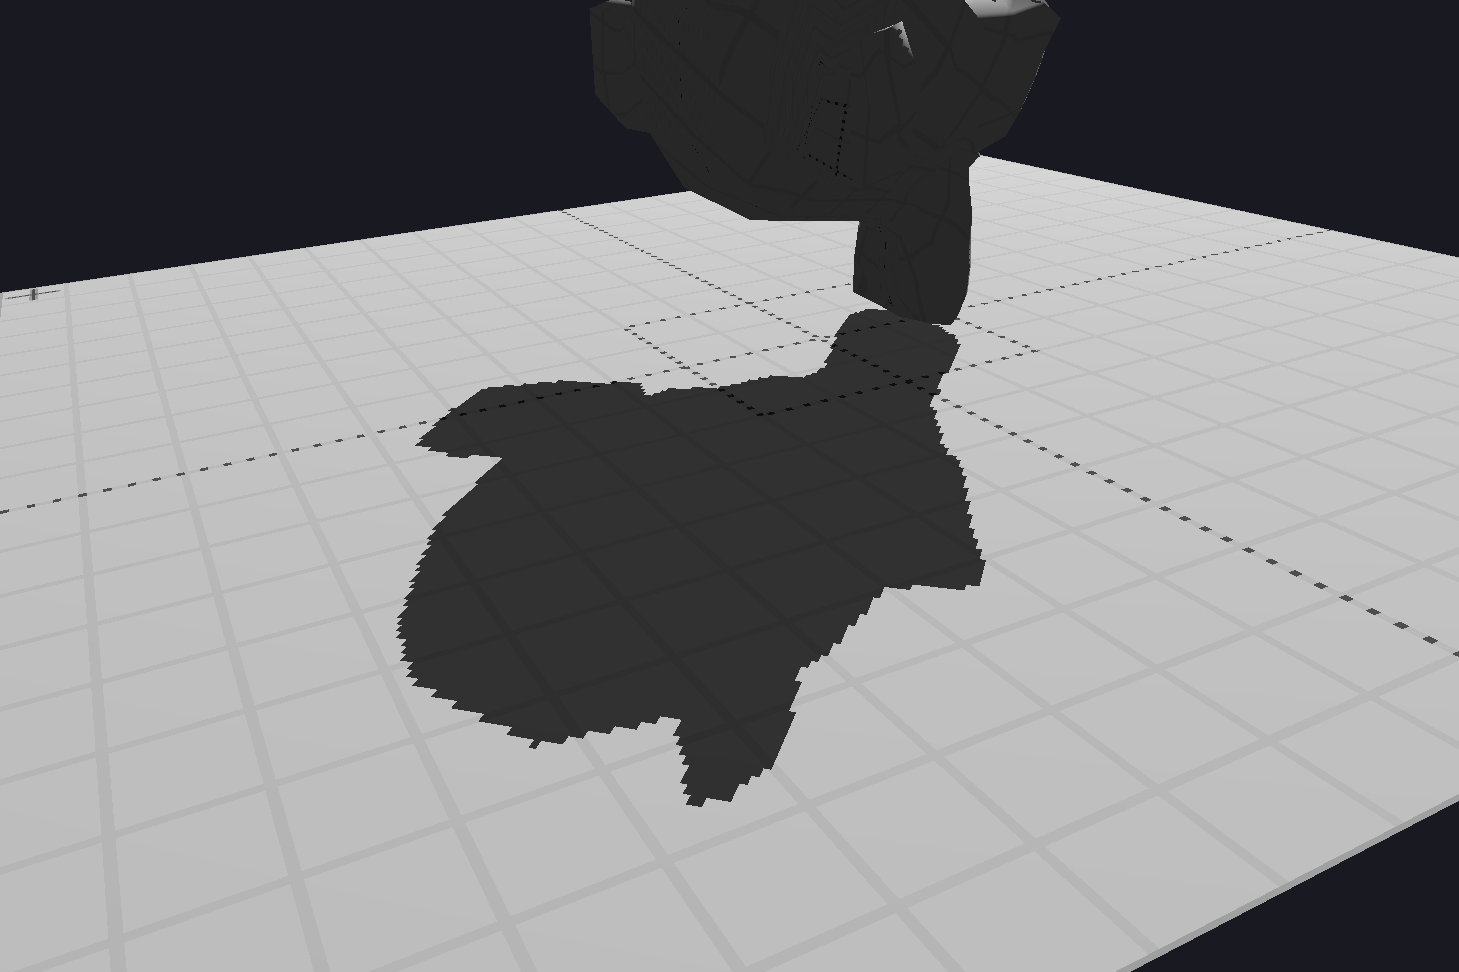
\includegraphics[width=0.7\textwidth]{./graf/shadow_mapping_blocky.png}
	\caption{Aliased shadow appearance due to no filtering and low resolution of the shadow map.}
	\label{fig:shadow_mapping_blocky}
\end{figure}

When rendering the shadow map an appropriate projection matrix has to be constructed. For a far away directional light, such as a sun light, an orthographic projection should be used. When rendering a spotlight a perspective projection can be used. Point lights can also use a single shadow map with a perspective projection matrix, but only in situations when the light source is positioned outside the scene, or at least is not surrounded by shadow casters. In the opposite case, the most common technique is to use cubemaps and improved derivative techniques as described by Liang Wan \cite{bib:article:wan_cubemaps}. A cubemap consists of six shadow map renders, each covering a face of a cube constructed around the light source. This way an omnidirectional shadow map is created.

When creating a projection matrix as well as the view matrix for a shadow map, care has to be taken to capture all relevant shadow casters. This is especially true for large scale scenes and directional lights, as rendering the entirety of a scene into the shadow map would most of the time be unnecessary and suboptimal. Most of the rendered map would not be used in a given frame, and the distribution of shadow map resolution would be poor. It would be enough for the light view to tightly encompass the view frustum of the observer to obtain correct results. This is called fitting and will be presented in the following sections. This idea can be taken further as shown by Ji\v{r}\'{\i} Bittner \cite{bib:proc:bittner_caster_culling} to allow for an approximate FPS gain of 1.5 times. Their method uses a custom advanced algorithm to cull shadow casters and render only those that contribute to the current main viewpoint.

Another issue of shadow maps is self-shadowing, or surface acne. This is also a result of aliasing, since the continuous scene geometry and its depth data is sampled in a discrete manner into an image when rendering the shadow map. If the shadow map texel does not correlate one-to-one with the final view samples, which happens very often and is highly likely, the shadow map samples will cover a non-zero area on the geometry surface in the final view of the scene, which is illustrated in Fig. \ref{fig:shadow_mapping_acne_explanation}.
\begin{figure}[hp]
	\centering
	\begin{subfigure}{0.7\textwidth}
        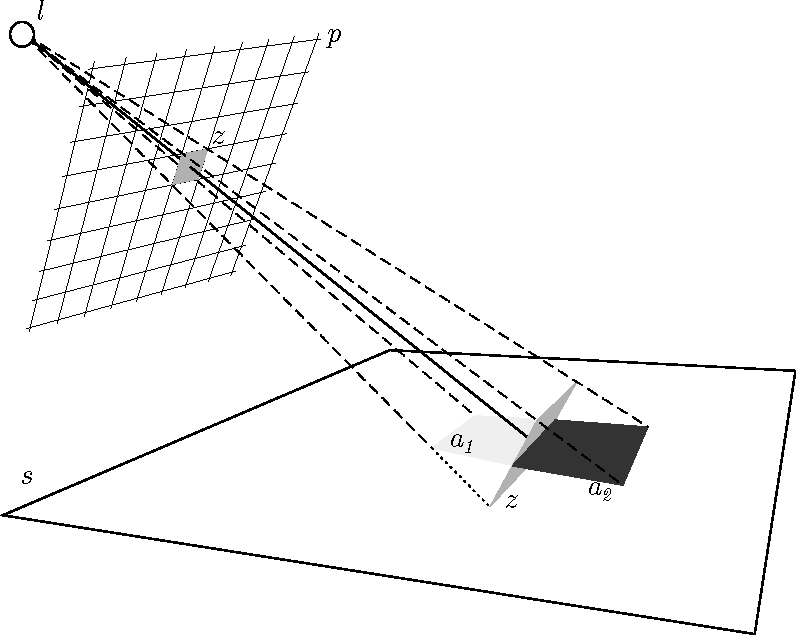
\includegraphics[width=\textwidth]{./graf/shadow_mapping_acne.pdf}
        \caption{Depth samples being compared with depth values over an area of the actual mesh lead to aliasing and shadow acne.}
        \label{fig:shadow_mapping_acne_explanation_3d}
    \end{subfigure}
	\begin{subfigure}{0.7\textwidth}
        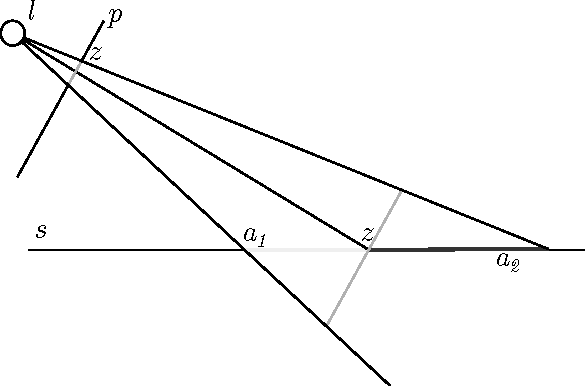
\includegraphics[width=\textwidth]{./graf/shadow_mapping_acne_side.pdf}
        \caption{The aliasing issue present in shadow maps illustrated in two dimensions from the side.}
        \label{fig:shadow_mapping_acne_explanation_side}
    \end{subfigure}

    \caption{The cause of shadow acne. Light source \(l\) renders the shadow map onto its projection plane \(p\), having some finite resolution. The sampled depth value \(z\) is stored in a texel. This creates a virtual surface orthogonal to the light direction on top of the actual geometry surface \(s\). When rendering the scene, depth values in the area \(a_1\) will have a lower depth value stored in the shadow map texel than their actual depth, causing them to be in light. Samples in the \(a_2\) area will have greater depth, causing them to be evaluated as being in shadow.}
    \label{fig:shadow_mapping_acne_explanation}
\end{figure}
This can cause the surface to erroneously shadow itself, as shown in Fig. \ref{fig:shadow_mapping_acne}. This issue gets more pronounced the higher the angle between the light source view ray and the surface normal. It can be resolved by adding a depth bias when rendering the shadow map, which will ensure the samples are below the actual surface. In modern rendering APIs the depth bias can be configured for a pipeline and applied automatically when rendering. Especially useful is the combination of a constant depth bias and a slope-scaled depth bias. The second bias helps eliminate the problem when surfaces appear more edge-on in the light view by scaling the depth bias with the angle between the light direction and surface. Too high depth bias can cause peter-panning, a situation shown in Fig. \ref{fig:shadow_mapping_panning} where a shadow caster gets detached from its shadow. Because of this, depth bias values often need to be hand-tuned on a per-scene basis. Other approaches have also been proposed, such as using only the back faces of objects to render the shadow map \cite{bib:rep:wang_second_depth_mapping} or utilizing depth peeling to store average depths between the back and front faces of an object \cite{bib:book:woo_midpoint_depth_map}, but they both still require some bias to avoid shadow-acne in areas such as silhouette edges or concavities.

\begin{figure}[h]
    \centering
    \begin{subfigure}{0.45\textwidth}
		\centering
        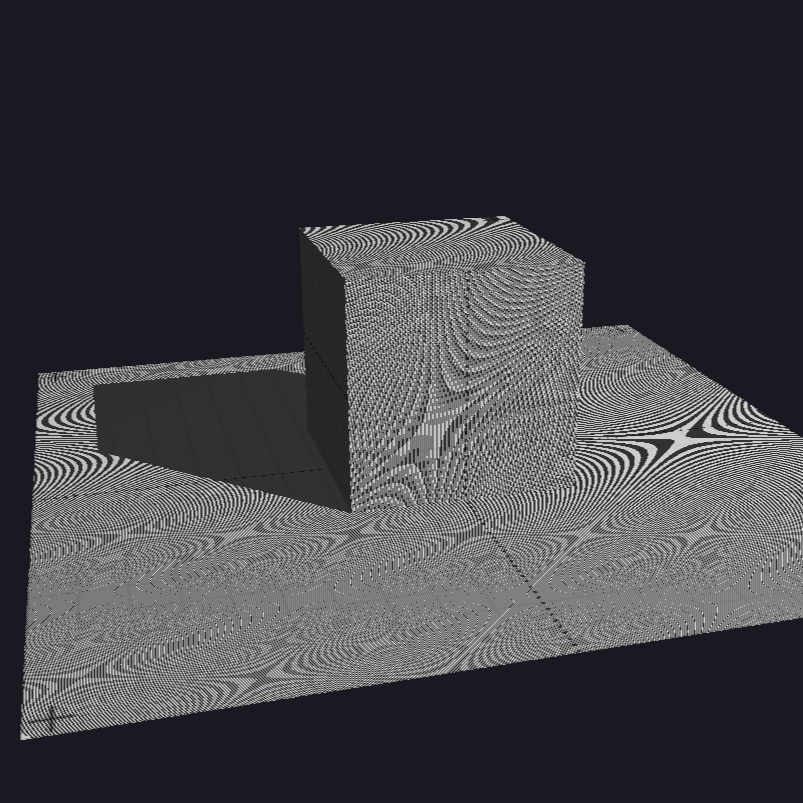
\includegraphics[width=\textwidth]{./graf/shadow_mapping_acne.png}
        \caption{Shadow acne due to using not enough bias.}
        \label{fig:shadow_mapping_acne}
    \end{subfigure}
	\hfill
    \begin{subfigure}{0.45\textwidth}
		\centering
        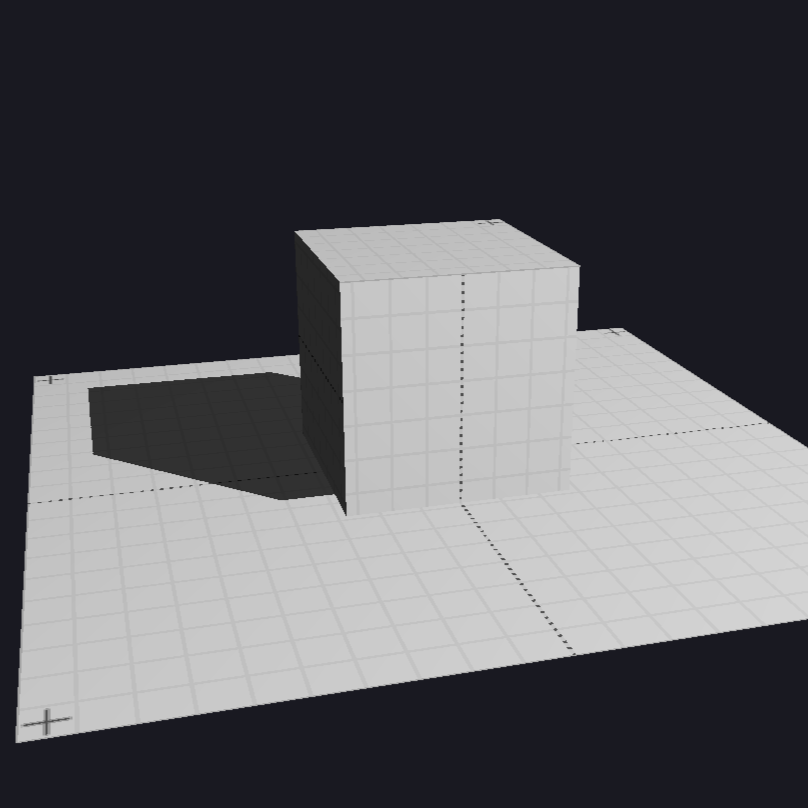
\includegraphics[width=\textwidth]{./graf/shadow_mapping_panning.png}
        \caption{The cube is disconnected from its shadow due to too much depth bias.}
        \label{fig:shadow_mapping_panning}
    \end{subfigure}

    \caption{Some of the issues that can arise when using projection shadows.}
    \label{fig:shadow_mapping_issues}
\end{figure}

The z-buffer of a rendered image can be actually non-linear in its \([0-1]\) range. Perspective projection matrices are sometimes built in such a way that the precision closer to \(1\) is lower than closer to \(0\). This is purposefully done to gain more precision closer to the viewer, where it is more needed when performing hidden-surface removal than far away, where objects will become very small due to perspective foreshortening. This can be an issue with shadow mapping, since objects close to the light source are not necessarily close to the viewer. In fact the opposite can often be true. As shown by Stefan Brabec \cite{bib:article:brabec_linear_depth}, the z-buffer for the use in shadow mapping can be linearized using a linear transformation dependent on the projection matrix used. The following perspective projection matrix present in the DX Math library can be linearized with equation \ref{eq:projection_linearization}.

\begin{gather}
	\label{eq:projection_perspective}
	\begin{pmatrix}
		W & 0 & 0 & 0\\
		0 & H & 0 & 0\\
		0 & 0 & \frac{f}{f-n} & \frac{-fn}{f-n}\\
		0 & 0 & 1 & 0
	\end{pmatrix}
    \begin{pmatrix}
		x\\
		y\\
		z\\
		w
	\end{pmatrix} =
    \begin{pmatrix}
		Wx\\
		Hy\\
		\frac{zf}{f-n} - \frac{wfn}{f-n}\\
		z
	\end{pmatrix} \Rightarrow 
    \begin{pmatrix}
		Wx\\
		Hy\\
		\frac{zf}{f-n} - \frac{fn}{f-n}\\
		z
	\end{pmatrix}
    \quad \text{for} \quad w = 1\\[10pt]
    \begin{pmatrix}
		Wx\\
		Hy\\
		\frac{zf}{f-n} - \frac{fn}{f-n}\\
		z
	\end{pmatrix} / z =
    \begin{pmatrix}
		\frac{Wx}{z}\\
		\frac{Hy}{z}\\
		\frac{f}{f-n} - \frac{fn}{z(f-n)}\\
		1
	\end{pmatrix}
\end{gather}

After the perspective division the final form of the z-value equation is obtained. Below, in Fig. \ref{plot:perspective_z}, the z-values are plotted for exemplary near and far clipping planes equal \(n=2\), \(f=15\).

\begin{figure}[h]
    \centering
    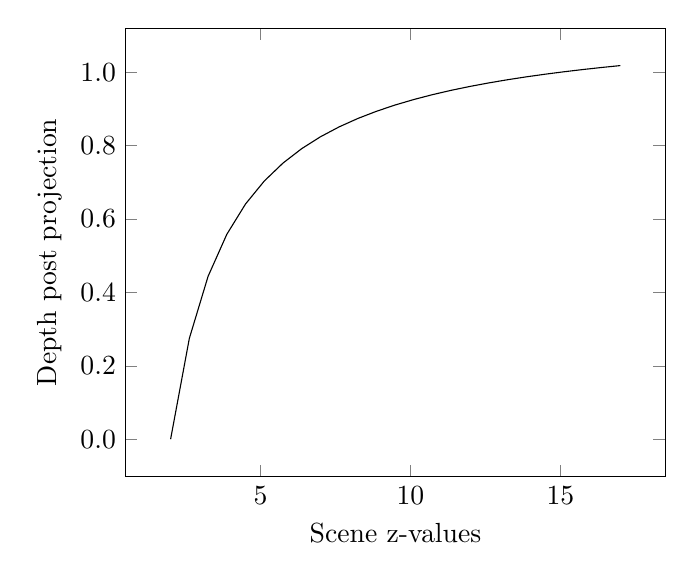
\begin{tikzpicture}
    \begin{axis}[
        xlabel=Scene z-values,ylabel=Depth post projection,
        y tick label style={
            /pgf/number format/.cd,
                fixed,   % po zakomentowaniu os rzednych jest indeksowana wykladniczo
                fixed zerofill, % 1.0 zamiast 1
                precision=1,
            /tikz/.cd
        },
        x tick label style={
            /pgf/number format/.cd,
                fixed,
                fixed,
                precision=2,
            /tikz/.cd
        }
    ]
    \addplot [domain=2.0:17.0] {(15/13)-(30/(13*x))};
    \end{axis} 
    \end{tikzpicture}
    \caption{The z-values after a perspective projection become non-linear.}
    \label{plot:perspective_z}
\end{figure}

The values can be linearized back again simply by multiplying the clip-space z-value by \(\frac{z}{f}\), which gives the following equation.

\begin{align}
	\label{eq:projection_linearization}
	\left(\frac{f}{f-n} - \frac{fn}{z(f-n)}\right) * \frac{z}{f} = \frac{z-n}{f-n}
\end{align}

In the application z-buffer linearization was not implemented, as after investigation it turned out that an orthographic projection, which is used for the directional light, does not introduce nonlinearity to the z-buffer range. This can be seen by inspecting how the matrix will affect the \(w\) component. The orthographic projection matrix as implemented in the DX Math library is presented below.

\begin{align}
	\label{eq:projection_ortho}
	\mathbf{M_{o}} = 
	\begin{pmatrix}
		W & 0 & 0 & 0\\
		0 & H & 0 & 0\\
		0 & 0 & \frac{1}{f-n} & \frac{-n}{f-n}\\
		0 & 0 & 0 & 1
	\end{pmatrix}
\end{align}

This matrix does not modify the \(w\) component and the \(z\) values will remain linear. In fact the formula for depth values after using this matrix is exactly the same as the perspective one after linearization.

\subsection{Fitting shadow maps}
An attempt to implement LiSPSM was made, but was not successful due to poor coverage of the implementation details both in the original paper and on the internet.

Only a part of the algorithm was implemented, basically providing simplified fitting of the shadow map view. The shadow map camera has certain extents set up by hand for each scene, such that the whole scene fits within view. Since the entire scene is not necessarily viewed at once by the observer, only the part that is within the observer view frustum can be rendered to the shadow map. Therefore, the shadow map post-projection space can be adjusted to include the area viewed by the observer.

This can be achieved by building a fitting transformation matrix \(\mathbf{F}\) that includes translation and scaling, that is applied after the light view and projection matrices, resulting in \(\mathbf{F}\mathbf{P}_L\mathbf{V}_L\). To obtain \(\mathbf{F}\), first the observer view frustum extents need to be found in world space, which can be obtained by applying the inverse of observer view and projection matrices to an NDC cuboid. This can be a cube with ranges \([-1:1]\) in \(x\), \(y\), \(z\) in APIs like OpenGL, or a cuboid with ranges \([-1:1]\) in \(x\) and \(y\), and \([0:1]\) in \(z\) in DirectX. Once the vertices of this cuboid are moved into world space, they can be multiplied by the view and projection matrices of the light source, \(\mathbf{P}_L\mathbf{V}_L\), and their components divided by \(w\) to bring them into the post-projection space of the light source. Once there, a bounding box can be found enclosing these points. To not move the contents of the shadow map beyond the original extent specified for the light source, the components of the vertices of this bounding box can be clamped to the NDC range. The whole process is shown in Fig. \ref{fig:shadow_map_fitting}.
\begin{figure}[hb]
    \centering
	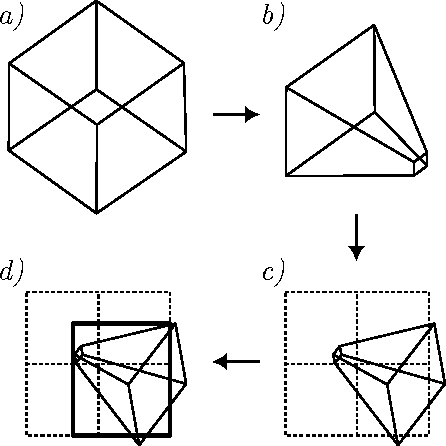
\includegraphics[width=0.5\textwidth]{./graf/shadow_map_focusing.pdf}
	\caption{The steps involved in fitting the shadow map. The NDC cuboid in a) is in observer post-projection space, or clip space. It is moved to the state presented in b) using inverse matrices, resulting in a world space representation of the viewing frustum. It is them transformed into c), the light view clipping space. Finally, a clamped bounding box is found, shown in d).}
	\label{fig:shadow_map_fitting}
\end{figure}
Finally, the minimum and maximum \(x\) and \(y\) values of these bounding vertices can be found and used in the following fitting matrix.
\begin{align}
	\mathbf{F} &= 
	\begin{pmatrix}
		s_x & 0 & 0 & o_x\\
		0 & s_y & 0 & o_y\\
		0 & 0 & 1 & 0\\
		0 & 0 & 0 & 1
	\end{pmatrix}, \text{where}\\[10pt]
	s_x &= \frac{2}{x_{max} - x_{min}} \quad\text{and}\quad o_x = \frac{-s_x(x_{max} + x_{min})}{2}
\end{align}
The calculation of \(s_y\) and \(o_y\) is analogous.

As was implemented, the fitting focuses on an approximate convex body of \(\mathbf{L}\cap \mathbf{V}\), where \(\mathbf{L}\) stands for the light view frustum and \(\mathbf{V}\) for the viewer frustum. The shadow map is then fitted only in the clip space \(x\) and \(y\) dimensions, ignoring depth \(z\). A more robust solution would be to find the convex hull of \(\mathbf{L}\cap \mathbf{V}\cap \mathbf{S}\), with \(\mathbf{S}\) meaning the scene bounding box. Then the shadow map would only focus on areas within the viewer frustum where there exists geometry to render. The near plane of the light frustum can then be set to the upper scene extent and the far plane to the farthest viewer frustum point. The shadow map would then require no hand adjustments to its frustum and would adapt to different scenes and viewer orientations.

\subsection{Filtering shadow maps with PCF}
\label{section:pcf}
As established in section \ref{section:filtering_shadow_maps}, percentage-closer filtering performs filtering of the shadow information to avoid aliasing artifacts. Basic shadow mapping performs a depth comparison giving a binary result on whether a scene point is in shadow of some other occluder or is directly in view of the light source. This comparison can be described with a formula \(s(t, z) = H(d(t) - z)\), where function \(s(t, z)\) is the shadow function that takes texture coordinates \(t\) and the depth value \(z\) of a scene sample in light space. Function \(d(t)\) is the depth lookup into the shadow map and \(H\) is the Heaviside function. This binary result can be obtained for positions near the initial scene sample and averaged, to get a value in the \([0:1]\) range describing how much light the point receives. This makes the technique relatively simple to implement in a renderer that already uses shadow mapping.

Possibly the simplest way to get PCF results is to use the hardware implementation made available by modern graphics APIs. This is accessible via the settings of the sampler that will be used with the shadow map. In DirectX 12 one can specify a linear comparison filter operation and a comparison function when creating a sampler. When later used in an HLSL shader, the SampleCmp function should be used. It takes the value to compare against as one of its arguments. It will perform comparison according to the comparison function with four nearest texels and bilinearly interpolate the results. The effect is shown in Fig. \ref{fig:pcf_methods_example}, in subfigure \ref{fig:pcf_bilinear}. This is done at practically no additional performance cost.

Unfortunately, hardware bilinear PCF is not going to significantly improve the shadow mapping visuals. In most cases there will still be visible aliasing, which is due to the fact that the kernel used is very small, being only \(2\times 2\). A larger kernel can be built manually and used in the same manner to get smoother shadows. A simple box filter with an \(n\times n\) kernel can cover a larger area in the shadow map. The larger the kernel, the smoother the shadow and the larger the penumbra. This can be implemented by generating an array of offsets either in the shader or, to preserve computing power, on the CPU and later sent to the GPU via a uniform buffer. The offsets should be in texel-aligned increments, which is easily achieved by expressing them in multiples of \(1/s\), where \(s\) is the shadow map size. These offsets are then added to the scene sample position expressed in light space. It is important to note, that even though different texels are sampled, the initial scene sample \(z\) value remains the same. Unfortunately, the visual quality of such filtering is visibly sub-par, as pixelated banding artifacts occur as shown in \ref{fig:pcf_manual}. This is due to the fact that only \(n^2+1\) shades can be obtained in the penumbra. The kernel size could obviously be raised, but sizes even as relatively low as 11 have a significant impact on performance. Hardware PCF can be used with this method to smooth out the banding as shown in Fig. \ref{fig:pcf_manual_with_bilinear}, and an offset scale can be utilized to control the size of the penumbra regardless of the size of the kernel.

A more robust and efficient approach allows using fewer samples while giving good visual results, sampling the shadow map adaptively. Instead of using a box filter it creates sets of randomly jittered offsets that are used when performing PCF. Most importantly, these offsets are stored in memory in such a way that allows to decide whether a point is fully lit or fully in shadow without having to test all samples. The offsets are first generated on the CPU in a jittered grid pattern of \(n\times n\) size. Their coordinates are normalized, so all samples lie within the \([0:1]\) range in the \(x\) and \(y\) axes. Then, all the samples are moved from the grid into a disk domain using the following equations.
\begin{align}
	u &= \sqrt{y} \times \cos(2\pi x)\\[10pt]
	v &= \sqrt{y} \times \sin(2\pi x)
\end{align}
The angular position of the sample on the disk is then determined by \(x\) and the \(y\) defines the radial distance from the center. If the loop that generates these points and stores them into an array is constructed in a smart way, the highest \(y\) coordinates are generated first, so the offsets the furthest away from the center are first in the array. This is then utilized in shader code when looping over the sample offsets and performing PCF: only the first \(n\) samples are tested at first, and if they all result in either \(0\) or \(1\), meaning the point is entirely in shadow or in light, further PCF processing for this point can stop. This delivers a significant performance boost, saving processing power where computations do not contribute to the visual outcome. The full set of samples will only be used in penumbras. The fact that all offsets have been normalized means that they can be multiplied by a scalar scale factor to control the amount of smoothing, or the size of the penumbra.

Unfortunately, the problem of banding in penumbra regions observed in simple box filtered PCF still persists. Hardware PCF can again be used to smooth the results further, but there is another solution to this problem. Instead of using a single set of jittered sample offsets, \(m\times m\) such sets can be generated and stored in a three-dimensional texture. In the shader this texture is accessed using the screen pixel coordinates, to choose a set of offsets, and then the set is indexed to perform PCF. This way banding is stochastically smoothed out in the final result, as shown in Fig. \ref{fig:pcf_random}. Creating an offset set for each pixel of the final image would consume a lot of memory and not provide significant gains, so small sets, such as \(16\times 16\) are used and tiled over the whole render area. This is enough to generate sufficient noise in the penumbra areas to create a smooth appearance.

\begin{figure}
    \centering
    \begin{subfigure}[t]{0.45\textwidth}
        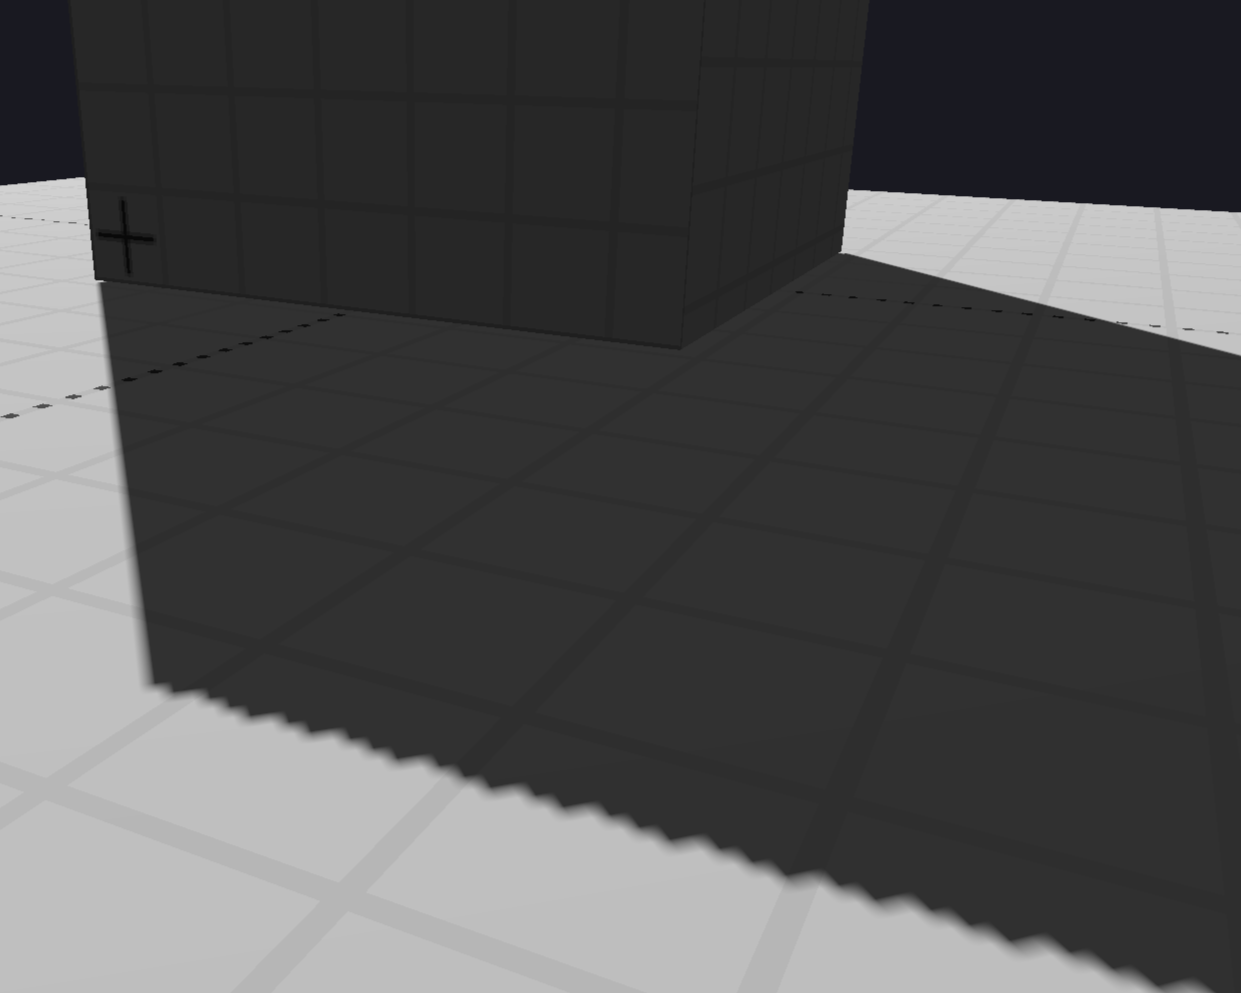
\includegraphics[width=\textwidth]{./graf/PCF_bilinear.png}
        \caption{Shadow mapping with hardware bilinear filtering.}
        \label{fig:pcf_bilinear}
    \end{subfigure}
    \hfill
    \begin{subfigure}[t]{0.45\textwidth}
        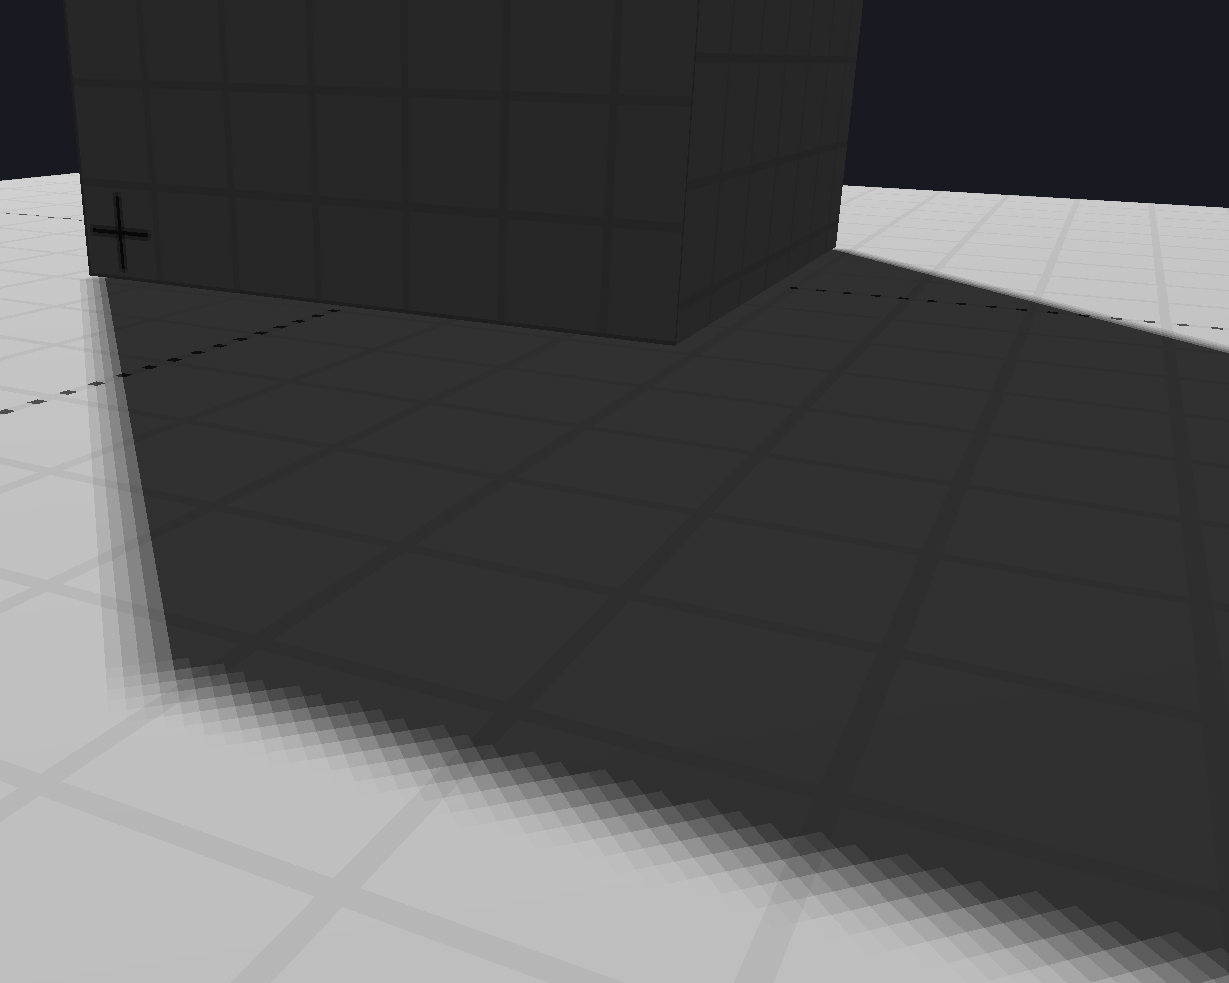
\includegraphics[width=\textwidth]{./graf/PCF_manual_kernel_5x5.png}
        \caption{Shadow mapping with a manually applied \(5\times 5\) kernel and box filter.}
        \label{fig:pcf_manual}
    \end{subfigure}

    \begin{subfigure}[t]{0.45\textwidth}
        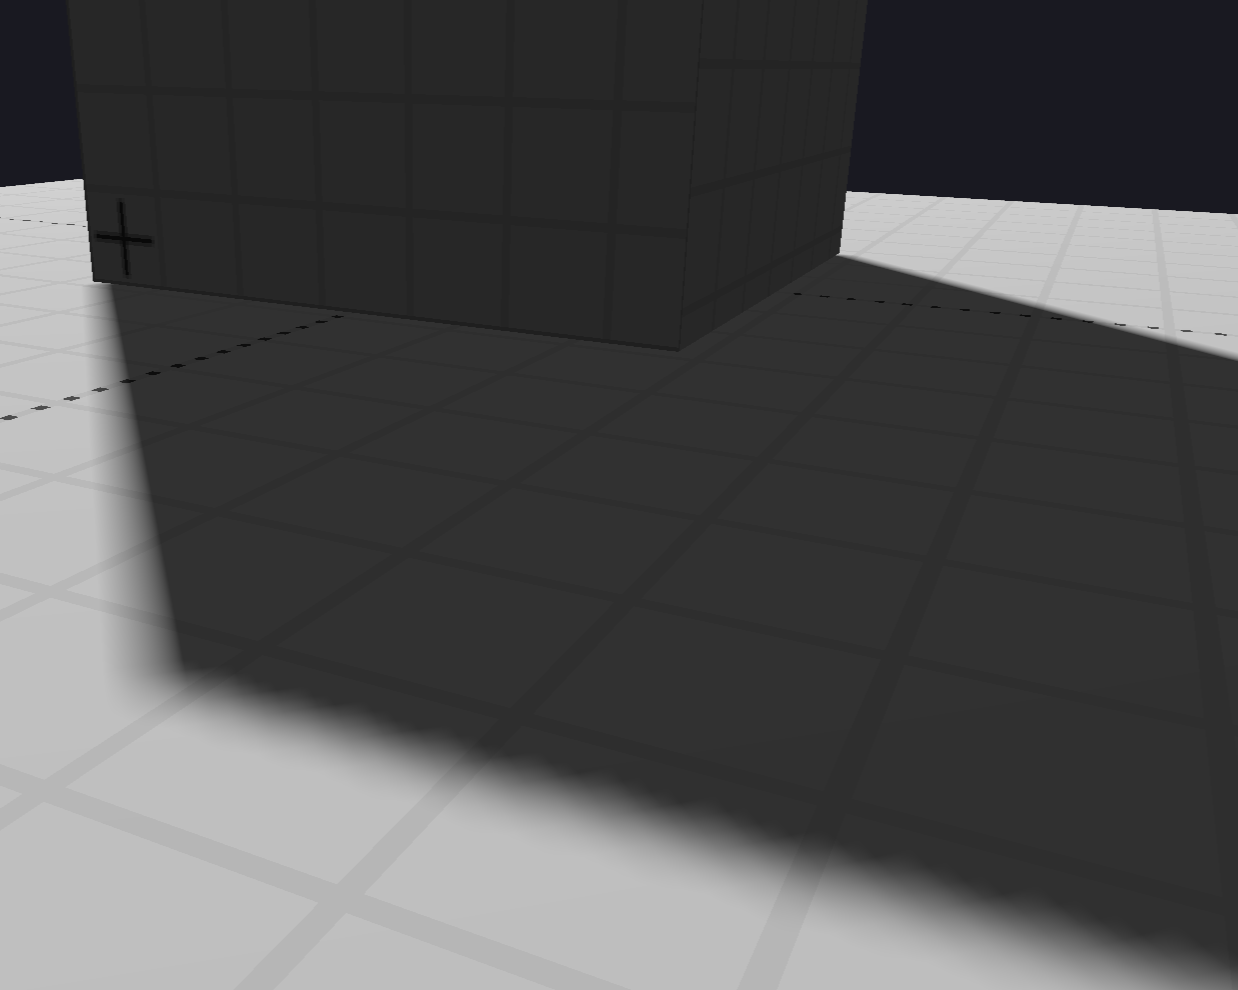
\includegraphics[width=\textwidth]{./graf/PCF_manual_kernel_5x5_bilinear.png}
        \caption{Shadow mapping with a manually applied \(5\times 5\) kernel and hardware bilinear filtering.}
        \label{fig:pcf_manual_with_bilinear}
    \end{subfigure}
    \hfill
    \begin{subfigure}[t]{0.45\textwidth}
        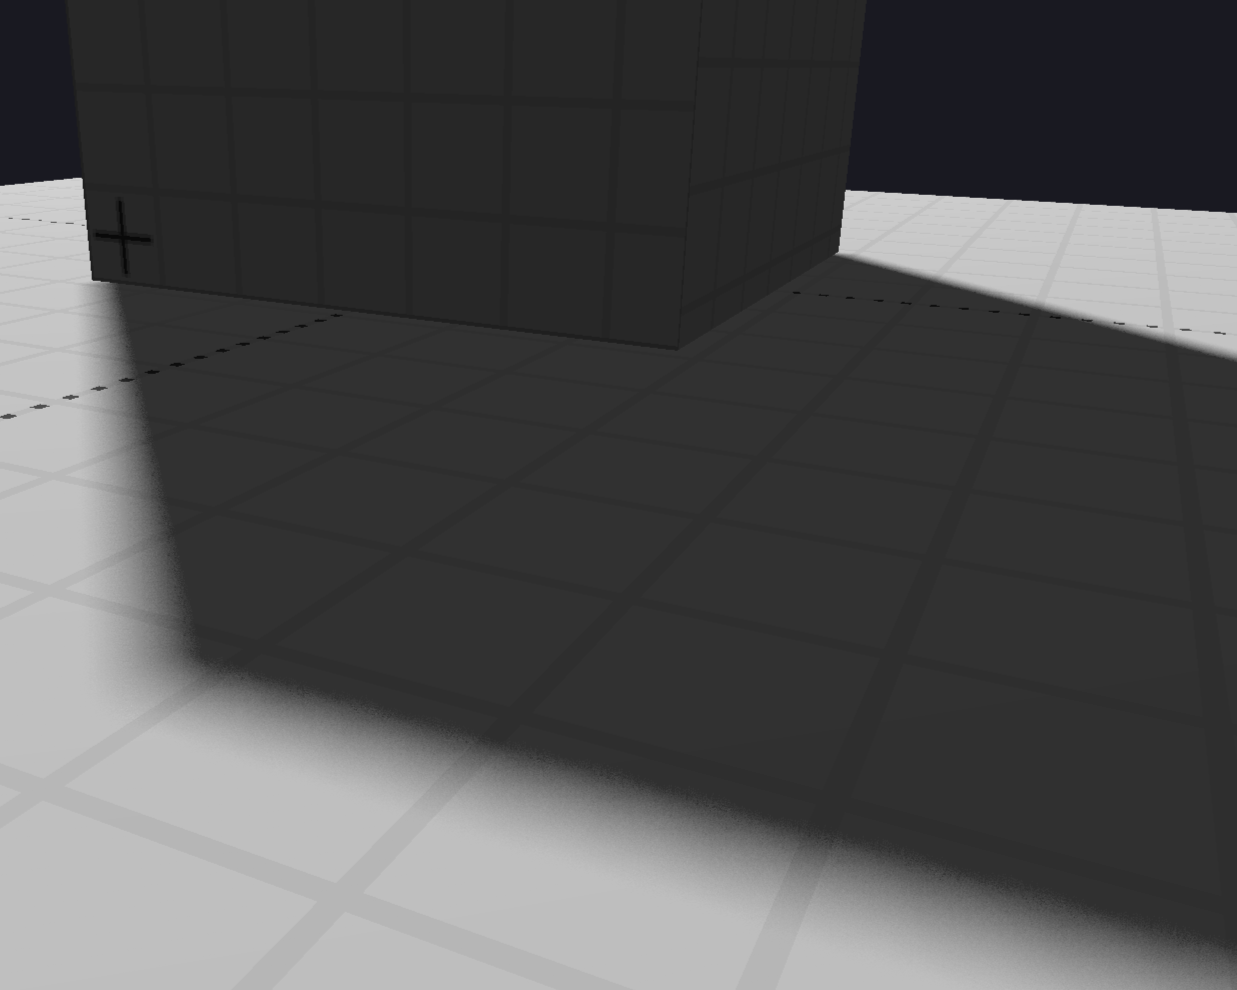
\includegraphics[width=\textwidth]{./graf/PCF_random_kernel_16x16_8x8.png}
        \caption{Shadow mapping with \(16\times 16\) sets of \(8\times 8\) jittered offsets.}
        \label{fig:pcf_random}
    \end{subfigure}
        
    \caption{Different results obtained with different PCF algorithms used to filter a \(512\times 512\) shadow map.}
    \label{fig:pcf_methods_example}
\end{figure}

As an argument against this technique one could point out the fact that GPU hardware does not handle dynamic branching well, and that it should be avoided to maintain the best performance. While this statement is generally true, it is not fully accurate. On modern GPUs the parallel threads that perform the computations run in groups, partially determined by their screen space positions, called warps or wavefronts. This is well explained and visualized by Nvidia in their developer article on the logical structure of the rendering hardware \cite{bib:internet:nvidia_traingle_life}. Since the branching in this algorithm depends on whether a pixel is in the penumbra region, it is dependent on screen space position and penumbra points will likely be in warps together, making the optimization effective.

A substantial problem of PCF algorithms is surface acne, which gets worse the larger the kernels and offset scales are used. This is because the sampled area of the shadow map increases and read depth values may vary more, while the depth of the scene point being shaded does not change. This can be again combated with a depth bias. An offset cone can be also used by applying higher bias the further from the original sample a point is. These however still need to be hand-tuned on a scene by scene basis. Additionally, it is important to note that, while PCF approaches do generate smooth shadows, they are not physically correct soft shadows. This is both due to the fact that the amount of smoothing is constant and that scene surface points are sampled. For an accurate shadow the area of the light source would need to be sampled for visibility from a given scene point, not the other way around.

\subsection{Implementing PCSS}
\label{section:pcss}
Percentage-closer soft shadows, as described in section \ref{section:soft_shadow_maps}, utilize the PCF technique and the fact that the shadows created with it can have varying levels of smoothness. The smoothness, or the size of the penumbra can be controlled by the kernel size and the scale of the sample offsets. When correctly driven, varying the size of the penumbra on a per-pixel basis can create plausible soft shadows that harden when close to the occluder. To achieve that, the estimated size of the penumbra has to be computed based on information about occluders and the size of the light source.

The algorithm first gathers information on the occluders that block the light source from the point of view of a point in the scene that is being shaded. For this a search radius is calculated from the following formula by projecting the base of a vision cone of the shaded point of the light source onto the shadow map.
\begin{align}
	s_{lv} &= \frac{s_{lw}}{s_{lf}} \label{eq:pcss_light_size} \\[10pt] 
	r &= s_{lv} \cdot \frac{p_{vz} - n}{p_{vz}}
\end{align}
In equation \ref{eq:pcss_light_size} \(s_{lv}\) is the size of the light source in light view space, \(s_{lw}\) is the size in world space and \(s_{lf}\) is the size of the light frustum. A square frustum is assumed, of size \(s_{lf}\times s_{lf}\). The sampling radius \(r\) is then calculated using the \(n\) - near clipping plane and \(p_{vz}\) being the \(z\) coordinate of the scene point in light view space, as illustrated in Fig. \ref{fig:shadow_map_pcss_search}. This search radius is then used to sample the shadow map in the area defined by \(r\) around the coordinates of the initial sample position in light space.
\begin{figure}[hb]
    \centering
	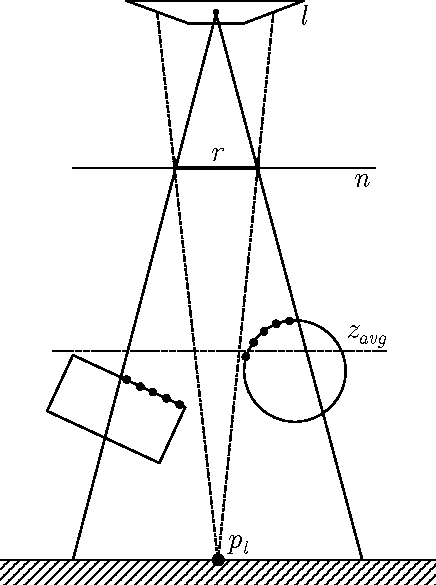
\includegraphics[width=0.33\textwidth]{./graf/shadow_mapping_pcss_search.pdf}
	\caption{The scene point in light view space \(p_l\) and its view cone marked in dashed lines project the area of the light source \(l\) onto the light frustum near plane \(n\). This creates the search radius \(r\) where depth samples are taken from the depth map, marked with black dots. These are averaged to obtain the average occluder depth \(z_{avg}\).}
	\label{fig:shadow_map_pcss_search}
\end{figure}
Sample offsets can be obtained in any way, as long as they are in the range \([0:1]\) and can be scaled with \(r\), for example using the sample offsets generated for adaptive PCF. The obtained depth values are averaged together and produce the average blocker depth \(z_{avg}\). Once this is known, the following formulas can be used to calculate the penumbra width, and from that the filter size.
\begin{align}
	s_{p} &= \frac{p_{vz} - z_{avg}}{z_{avg}}s_{lv} \label{eq:pcss_penumbra} \\[10pt] 
	s_f &= \frac{n}{p_{vz}}s_{p}
\end{align}
Equation \ref{eq:pcss_penumbra} calculates the penumbra size \(s_{p}\) and is based on similar triangles. Then the filter size \(s_f\) can be derived. This can be directly used for performing PCF.

The size of the penumbras is not dependent on the resolution of the shadow map thanks to equation \ref{eq:pcss_light_size}. PCSS however does have its problems. It is not practical to perform the occluder search exhaustively, so the number of samples needs to be carefully chosen to avoid undersampling and give meaningful estimates. The amount of depth map texture lookups is even higher than with PCF, which puts a strain on texture memory bandwidth. The contact-hardening shadows that it produces are not physically correct. This is in part due to the fact that the algorithm uses the average depth of occluders and assumes that the average occluder, light and receiver are planar and parallel. Additionally, shadow map samples taken for averaging often stretch beyond the shadow map area containing the actual occluders.


% \begin{itemize}
% \item solution to the problem proposed by the author of the thesis
% \item theoretical analysis of proposed solutions
% \item rationale of applied methods, algorithms, and tools
% \end{itemize}

% Here I should describe my reasoning for the testing, reasoning for
% selecting the techniques that I do select, my program for testing.

% \section{[Section title]}

% \section{[Subsection title]}

% Each figure in the document should be referred to at least once (fig. \ref{fig:2}).

% \begin{figure}
% \centering
% \begin{tikzpicture}
% \begin{axis}[
%     y tick label style={
%         /pgf/number format/.cd,
%             fixed,   % po zakomentowaniu os rzednych jest indeksowana wykladniczo
%             fixed zerofill, % 1.0 zamiast 1
%             precision=1,
%         /tikz/.cd
%     },
%     x tick label style={
%         /pgf/number format/.cd,
%             fixed,
%             fixed zerofill,
%             precision=2,
%         /tikz/.cd
%     }
% ]
% \addplot [domain=0.0:0.1] {rnd};
% \end{axis} 
% \end{tikzpicture}
% \caption{Figure caption.} % Figure caption is BELOW the figure!
% \label{fig:2}
% \end{figure}


%%%%%%%%%%%%%%%%%%%%%
% FIGURE FROM FILE
%
%\begin{figure}
%\centering
%
\includegraphics[width=0.5\textwidth]{./graf/politechnika_sl_logo_bw_pion_en.pdf}
%\caption{Caption of a figure is always below the figure.}
%\label{fig:label}
%\end{figure}
%Fig. \ref{fig:label} presents …
%%%%%%%%%%%%%%%%%%%%%
%
%%%%%%%%%%%%%%%%%%%%
%% SUBFIGURES
%
%\begin{figure}
%\centering
%\begin{subfigure}{0.4\textwidth}
%    
\includegraphics[width=\textwidth]{./graf/politechnika_sl_logo_bw_pion_en.pdf}
%    \caption{Upper left figure.}
%    \label{fig:upper-left}
%\end{subfigure}
%\hfill
%\begin{subfigure}{0.4\textwidth}
%    
\includegraphics[width=\textwidth]{./graf/politechnika_sl_logo_bw_pion_en.pdf}
%    \caption{Upper right figure.}
%    \label{fig:upper-right}
%\end{subfigure}
%
%\begin{subfigure}{0.4\textwidth}
%    
\includegraphics[width=\textwidth]{./graf/politechnika_sl_logo_bw_pion_en.pdf}
%    \caption{Lower left figure.}
%    \label{fig:lower-left}
%\end{subfigure}
%\hfill
%\begin{subfigure}{0.4\textwidth}
%    
\includegraphics[width=\textwidth]{./graf/politechnika_sl_logo_bw_pion_en.pdf}
%    \caption{Lower right figure.}
%    \label{fig:lower-right}
%\end{subfigure}
%        
%\caption{Common caption for all subfigures.}
%\label{fig:subfigures}
%\end{figure}
%Fig. \ref{fig:subfigures} presents very important information, eg. Fig. \ref{fig:upper-right} is an upper right subfigure.
%%%%%%%%%%%%%%%%%%%%%


% Each table in the document should be referred to at least once (Tab. \ref{tab:results}).

% \begin{table}
% \centering
% \caption{A caption of a table is ABOVE it.}
% \label{tab:results}
% \begin{tabular}{rrrrrrrr}
% \toprule
% 	         &                                     \multicolumn{7}{c}{method}                                      \\
% 	         \cmidrule{2-8}
% 	         &         &         &        \multicolumn{3}{c}{alg. 3}        & \multicolumn{2}{c}{alg. 4, $\gamma = 2$} \\
% 	         \cmidrule(r){4-6}\cmidrule(r){7-8}
% 	$\zeta$ &     alg. 1 &   alg. 2 & $\alpha= 1.5$ & $\alpha= 2$ & $\alpha= 3$ &   $\beta = 0.1$  &   $\beta = -0.1$ \\
% \midrule
% 	       0 &  8.3250 & 1.45305 &       7.5791 &    14.8517 &    20.0028 & 1.16396 &                       1.1365 \\
% 	       5 &  0.6111 & 2.27126 &       6.9952 &    13.8560 &    18.6064 & 1.18659 &                       1.1630 \\
% 	      10 & 11.6126 & 2.69218 &       6.2520 &    12.5202 &    16.8278 & 1.23180 &                       1.2045 \\
% 	      15 &  0.5665 & 2.95046 &       5.7753 &    11.4588 &    15.4837 & 1.25131 &                       1.2614 \\
% 	      20 & 15.8728 & 3.07225 &       5.3071 &    10.3935 &    13.8738 & 1.25307 &                       1.2217 \\
% 	      25 &  0.9791 & 3.19034 &       5.4575 &     9.9533 &    13.0721 & 1.27104 &                       1.2640 \\
% 	      30 &  2.0228 & 3.27474 &       5.7461 &     9.7164 &    12.2637 & 1.33404 &                       1.3209 \\
% 	      35 & 13.4210 & 3.36086 &       6.6735 &    10.0442 &    12.0270 & 1.35385 &                       1.3059 \\
% 	      40 & 13.2226 & 3.36420 &       7.7248 &    10.4495 &    12.0379 & 1.34919 &                       1.2768 \\
% 	      45 & 12.8445 & 3.47436 &       8.5539 &    10.8552 &    12.2773 & 1.42303 &                       1.4362 \\
% 	      50 & 12.9245 & 3.58228 &       9.2702 &    11.2183 &    12.3990 & 1.40922 &                       1.3724 \\
% \bottomrule
% \end{tabular}
% \end{table}  


% \begin{figure}
% \centering
% 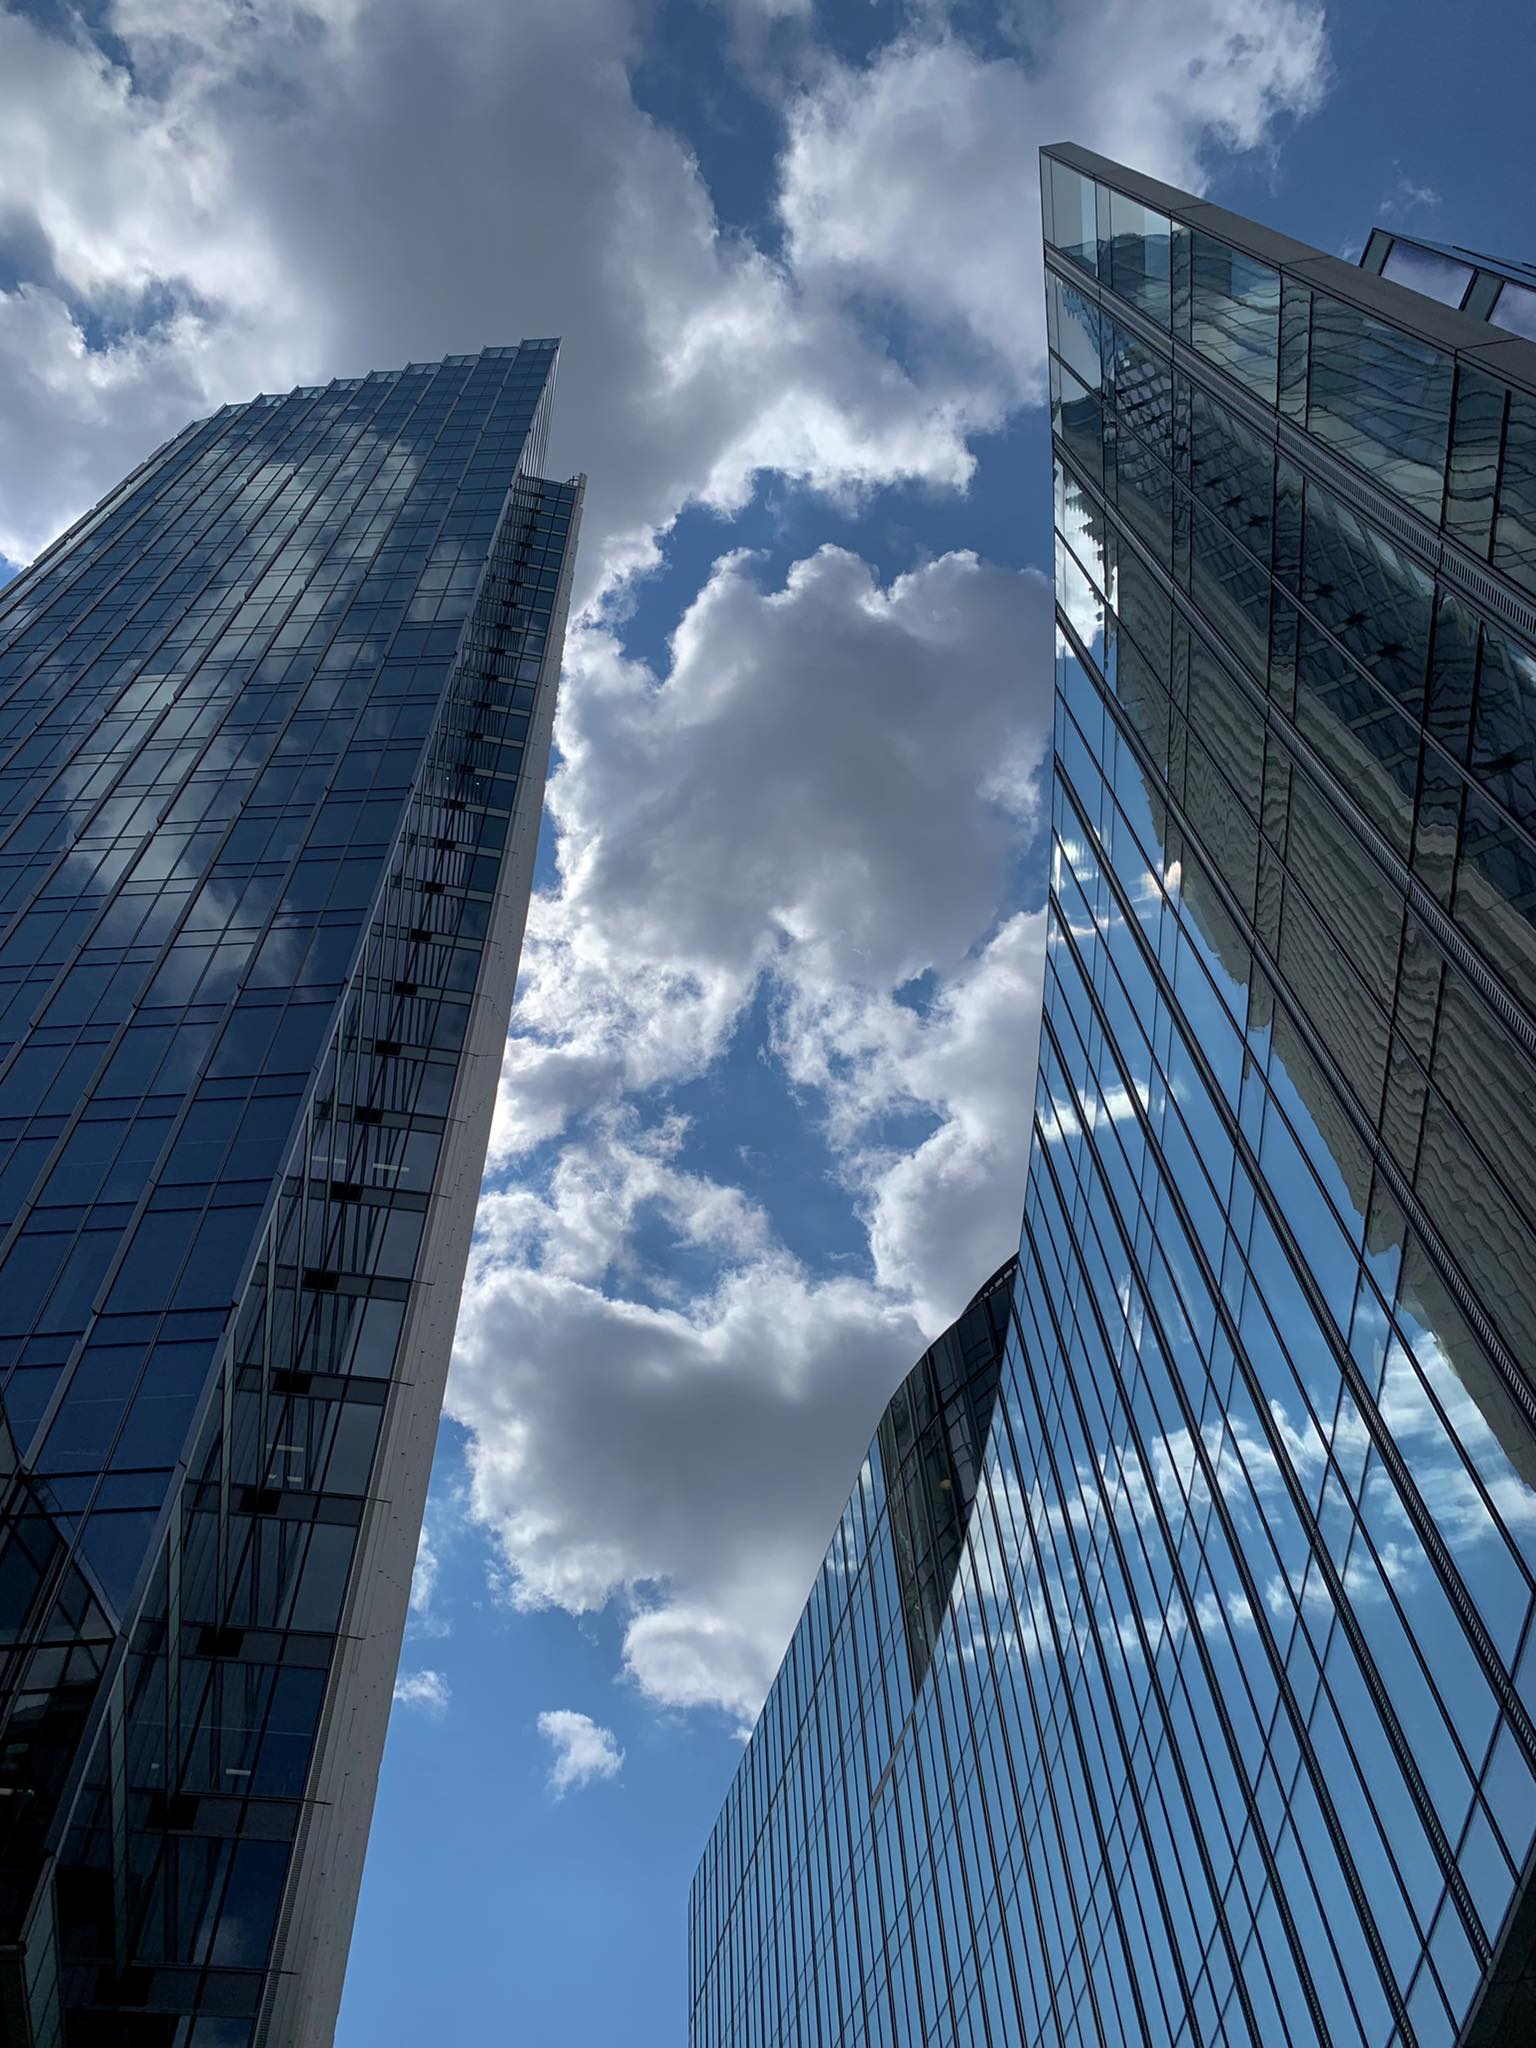
\includegraphics[width=0.5\textwidth]{./graf/test_image.jpg}
% \caption{Caption of a figure is always below the figure akakak.}
% \label{fig:duped_image4}
% \end{figure}

% some citation of the above \ref{fig:duped_image4}
